\label{sec:nuc}

%The majority of the nuclei produced since the Big Bang have been
%produced through processes that involve stars {\bf citation?}.  One
%notable exception to this is cosmic rays, which produce elements such
%as Li, Be, and B (\citealt{meneguzzi1971}) and isotopes such as
%$^{14}$C.  
The classical picture of stellar nucleosynthesis is of main
sequence stars
building H into $^4$He in their cores then, in subsequent stages of
evolution, producing the various stable $\alpha$-nuclei up to 
and including $^{56}$Ni. This pathway only accounts for a small fraction of all the elements
that exist in the universe and only one of multiple isotopes for each
element created by this pathway.  To fully
understand the chemical evolution of stars, galaxies, and the universe
we must understand the other processes involved in nucleosynthesis.

\begin{figure}
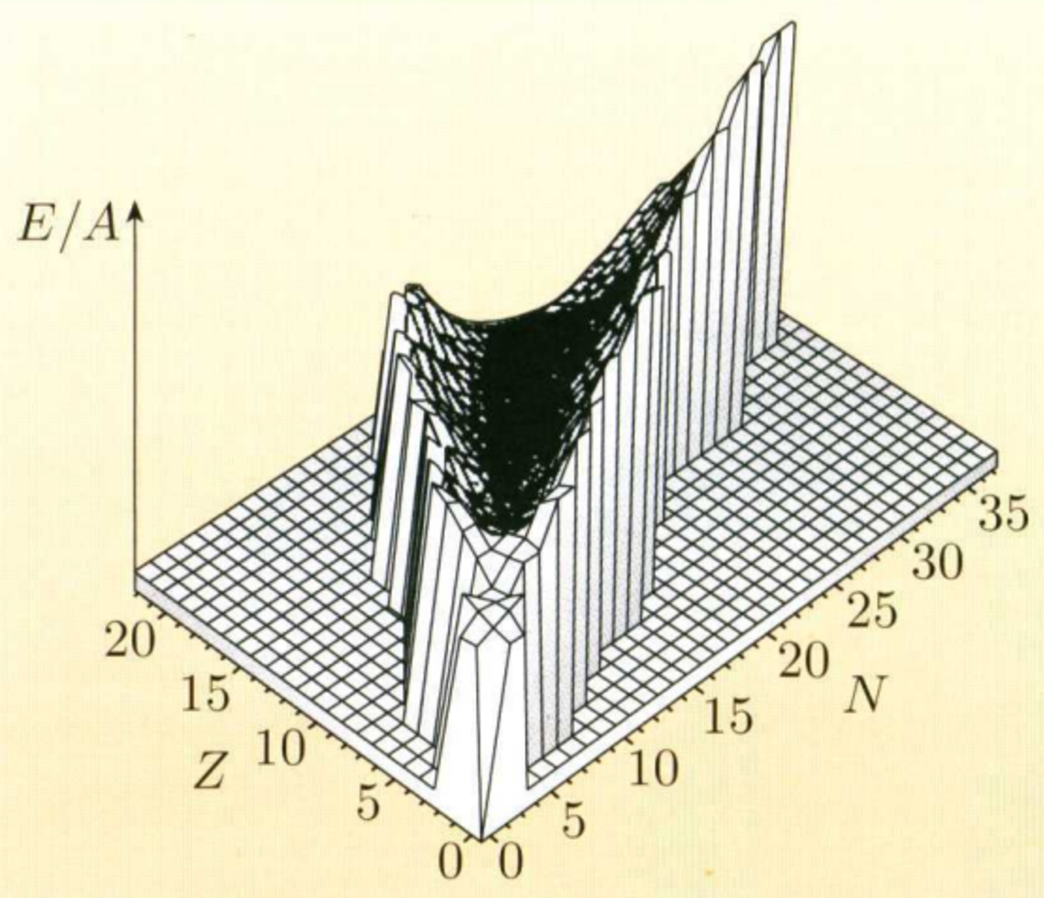
\includegraphics[width=\linewidth]{pdf/con.png}
\caption{\label{fig:con} The Chart of the Nuclides, showing the
  binding energy per nucleon for various combinations of atomic number
  $Z$ and number of neutrons $N$.  The valley of stability is shown as
  the minimum in the binding energy per nucleon region. From~\cite{ryan2010}.}
\end{figure}

\begin{figure}
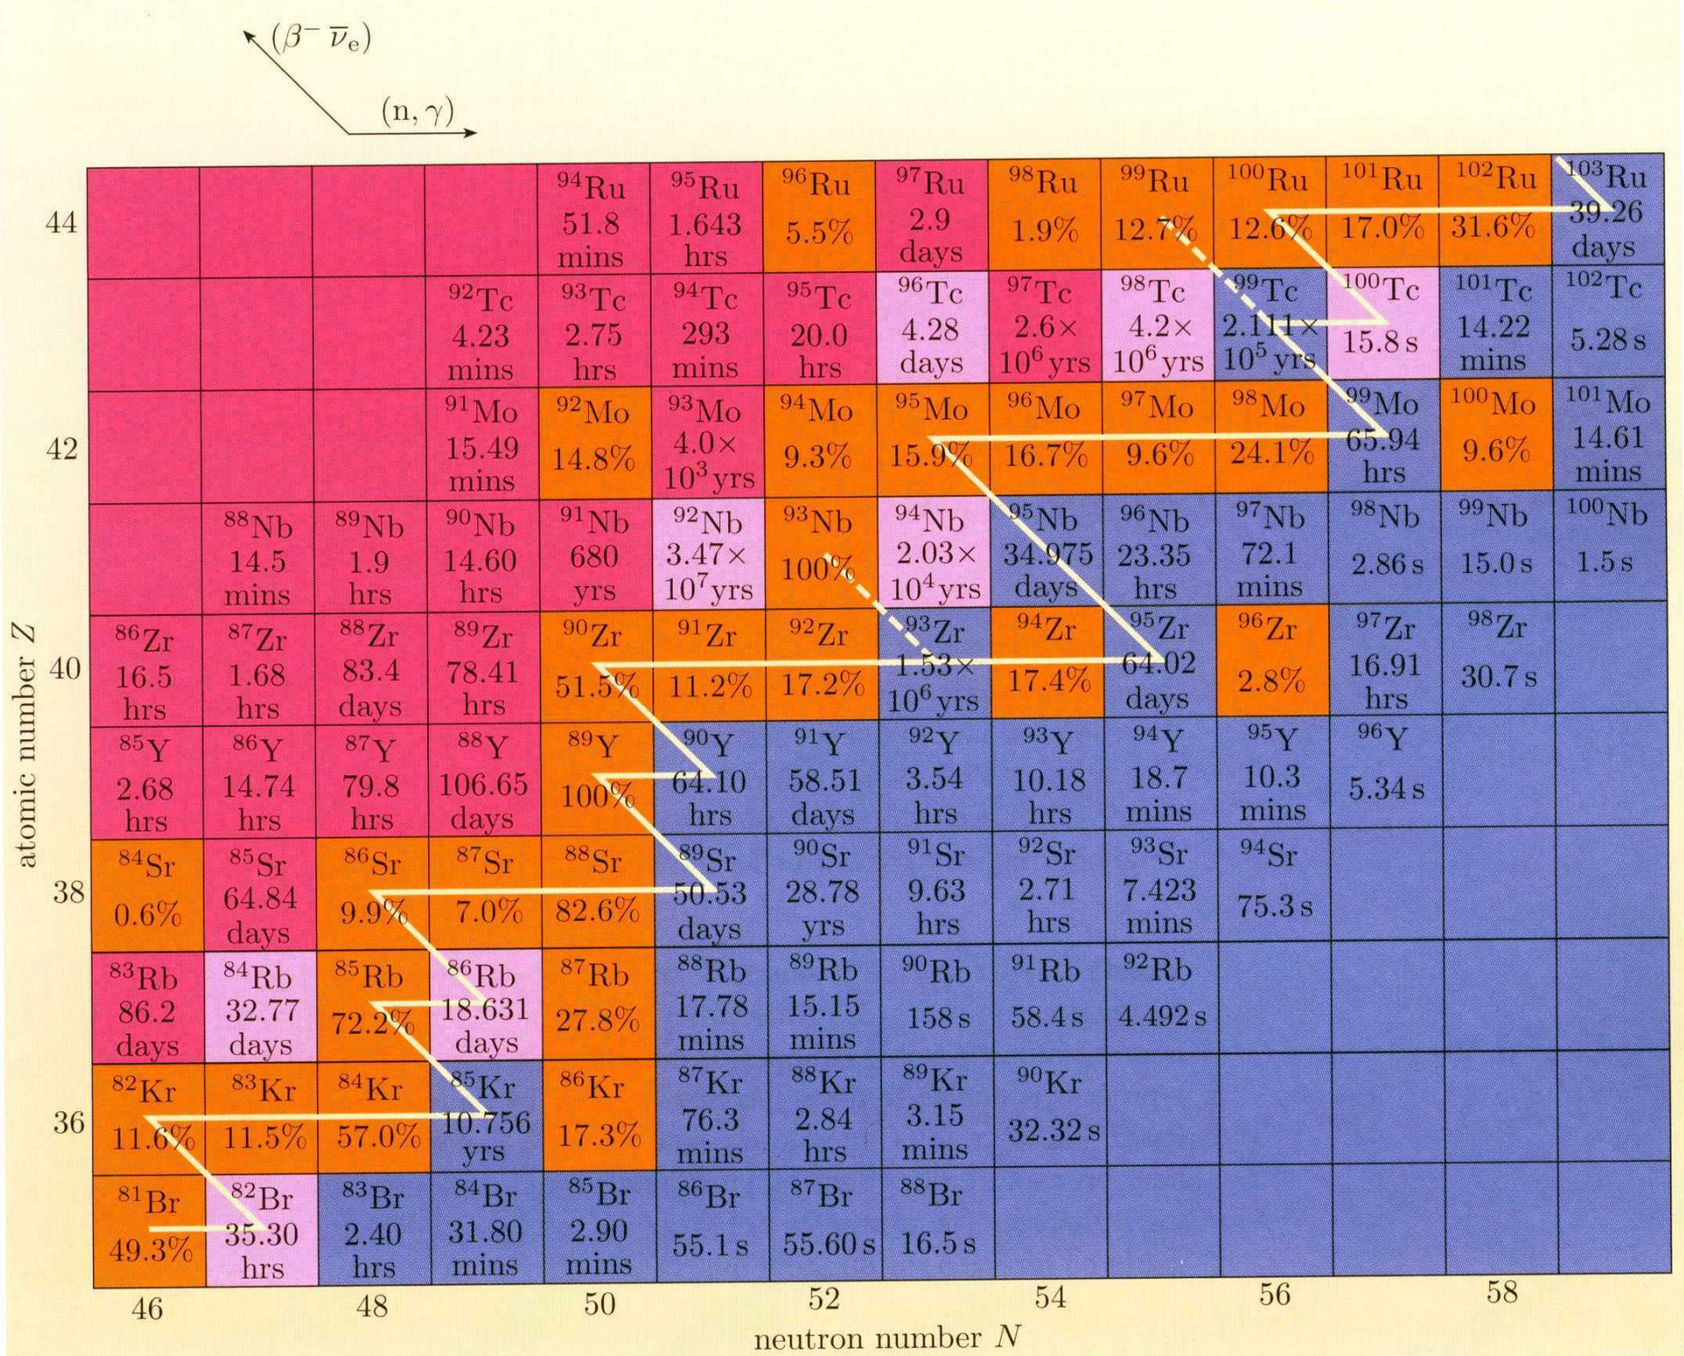
\includegraphics[width=\linewidth]{pdf/con2.png}
\caption{\label{fig:con2} A zoom in of a section of the CON, for
  $35\leq Z \leq 44$ and neutron number $46\leq N \leq 59$.  Orange shows stable
  nuclides, light pink (such as $^{86}$Rb) shows nuclides that either
  \bminus\ decay or electron capture, dark pink shows nuclides that
  electron capture, and blue show nuclides that \bminus\ decay.
  Percentages on stable nuclides represent relative contribution to
  measured solar system abundances.  Time on the unstable nuclides
  represent their half-life.  An s-process reaction pathway is shown
  (to be discusses in Section~\ref{sec:s}). Steps taken on the CON by
  two specific nuclear reactions are shown in the upper left.  From~\cite{ryan2010}.}
\end{figure}
I first introduce some relevant physics.  Figure~\ref{fig:con}
shows what is referred to as the ``Chart of the Nuclides'' (hereafter
CON), which
shows all the nuclides as well as their stability.  The axis going diagonal left represents the atomic number $Z$ while the
axis going diagonal right represents the neutron number $N$.  The
so-called valley of stability is shown as a minimum in the binding
energy per nucleon, which in this figure stands as a proxy for nuclear
stability. Nuclei that do not lie on this valley of stability tend to
undergo nuclear decays that move them closer to the valley of
stability.  Figure~\ref{fig:con2} shows a section of the CON in
greater detail.  Nuclides on the high neutron side (shown in blue) of the valley of
stability (shown in orange) tend to \bminus\ decay to the valley of
stability.  Species of the
same $A=Z+N$ are positioned to the upper left and lower right from
each other.  Nuclear reactions can be represented bas specific steps in
the CON.  Most relevant to this work are the neutron
capture and \bminus\ decay reactions.  Steps on the CON taken by these
reactions are represented by the arrows in the upper left of
Figure~\ref{fig:con2}.
  Neutron capture on a given
species $^{A}_ZX$ is given by
\begin{equation}
\label{eq:nc}
^{A}_ZX + n \rightarrow ^{A+1}_{\ \ \ Z}X' + \gamma
\end{equation}
and is represented in the CON by a step from species $^{A}_ZX$ to the
species directly to the right of it.  Similarly, \bminus\ decay of a
given species $X$ is given by
\begin{equation}
\label{eq:bd}
^{A}_ZX  \rightarrow ^{\ \ \ A}_{Z+1}X' + e^- + \overline{\nu}_e
\end{equation}
and is represented in the CON by a step from species $X$ to the
species immediately up and the left of it.  For the r- and s-processes
these are the most important steps in the CON.

The r- and s-process are both involve neutron capture.  This is
significant because neutrons have a relatively short half-life; thus
the presence of free neutrons, required for neutron capture, depends
on there being a ready source of neutrons.  Additionally, the free
neutron density is highly dependent on the details of the neutron
source, because decaying neutrons need to be replenished to maintain a
given density.

Also important to the r- and s-process are the nuclear magic numbers.
Nuclides with neutron numbers equal to one of these magic numbers are
more stable than other nuclides close to them in ($Z$,$A$) space.
These magic numbers include 2, 8, 20, 28, 50, 82, and 126, with the
latter three numbers being most relevant to the examination of this
paper.  Nuclides with these magic numbers of neutrons also have 
smaller neutron capture cross-sections, which affects the
relative abundances of nuclides produced by these processes.  The
specifics will be discussed in Sections~\ref{sec:s} and~\ref{sec:r}.
It should be noted that protons also have the same magic numbers;
nuclei with a magic number of both protons and neutrons are called
``doubly magic'' and are even more stable than singly magic nuclei.  

It should also be mentioned that many of the stable proton-rich
nuclides are formed via proton capture (through what is known as the p-process).  
Figure~\ref{fig:con2} shows an example of such a nuclide, $^{92}_{42}$Mo.  This paper will not focus
on any discussion of p-processed nuclides and such nuclides will not
figure in my discussions.

%  LocalWords:  nuc meneguzzi1971 bminus nc
